\PassOptionsToPackage{quiet}{fontspec}
\documentclass[12pt,a4paper,UTF8]{article}
\usepackage{thesis} % 格式控制
\usepackage{indentfirst}
\setlength{\parindent}{2em} % 控制首行缩进
\addtolength{\parskip}{3pt} % 控制段落距离
\onehalfspacing % 1.5倍行距
\graphicspath{{./figures/}} % 指定图片所在文件夹
\pagestyle{empty}
\usepackage{enumitem}
\usepackage{multirow}
\usepackage{makecell}
\usepackage{float}

\classname{算法设计与智能计算}  % 设置课程名称

\begin{document}
\maketitlepage{基于MindSpore的MNIST手写体数字识别实验(卷积神经网络)}{施景皓}{3230100613}{2026.6.4}{Min Li} % 封面页

\newpage

\pagestyle{fancy}
\fancyhf{}
\lhead{算法大作业}
\chead{基于MindSpore的MNIST手写体数字识别}
\rhead{施景皓\ 3230100613}
\renewcommand{\headrulewidth}{0.4pt}
\cfoot{\thepage}

\maketoc    % 目录页

\section{实验目的}

本次实验全名为“基于 MindSpore 的 MNIST 手写体数字识别实验（卷积神经网络）”，以 MNIST 手写数字识别为任务背景，在华为云 ModelArts 平台上使用 MindSpore 框架完成卷积神经网络的训练与测试。实验主要围绕 MindSpore 中数据集读取、数据预处理、CNN 网络构建、损失函数定义、优化器配置、模型训练、测试评估和预测可视化等流程展开，并进一步理解卷积神经网络在图像分类任务中的应用方法。

在完成基础实验的过程中，报告重点关注 LeNet-5 网络的结构组成和前向计算过程，并结合训练结果分析 epoch、平均损失和测试准确率之间的变化关系。除此之外，还在原始 LeNet-5 的基础上调整部分网络结构，并将改进模型与原始模型放在相同条件下进行比较，以观察网络结构变化对识别效果的影响。

\section{实验任务}

本次大作业的基本要求是参考华为《人工智能程序设计》实验内容完成一个基于 MindSpore 的实验，并在报告中整理实验过程、实验数据和数据分析。本报告选择“基于 MindSpore 的 MNIST 手写体数字识别实验（卷积神经网络）”，主要完成 MNIST 数据集下载、数据预处理、LeNet-5 卷积神经网络模型训练、测试评估和预测结果展示。

在原始实验的基础上，报告增加了一个改进实验：保持 MNIST 数据集、训练轮数、损失函数和优化器设置一致，只调整 LeNet-5 的部分网络结构，然后比较原始模型和改进模型的训练结果，分析结构变化对测试准确率和平均损失值的影响。

\section{实验环境}

本次实验在华为云 ModelArts 平台上完成，开发环境为在线 Notebook。创建 Notebook 时选择公共镜像中的 MindSpore 2.2 环境，对应 Python 3.9、CANN 7.0.1、EulerOS 2.10.7 和 aarch64 架构。硬件资源类型为 Ascend，实例规格为 1 个 Ascend 处理器并配套 ARM CPU 资源。

实验过程中通过 JupyterLab 打开并运行 notebook 文件。主要源文件位于 \texttt{src} 目录下，包括原始实验 notebook 和改进实验 notebook。其中，原始 notebook 用于完成 LeNet-5 卷积神经网络的训练、测试与预测可视化，改进 notebook 则在相同流程基础上补充了改进版 LeNet-5 的训练和对比实验。

ModelArts Notebook 创建配置如图~\ref{fig:modelarts-config} 所示。创建环境时开启了自动停止功能，停止时长设置为 1 小时。由于云硬盘 EVS 从 Notebook 实例创建成功开始计费，并且会持续到实例删除成功为止，所以实验完成后及时停止并清理了 Notebook，避免继续产生不必要的费用。

\begin{figure}[H]
  \centering
  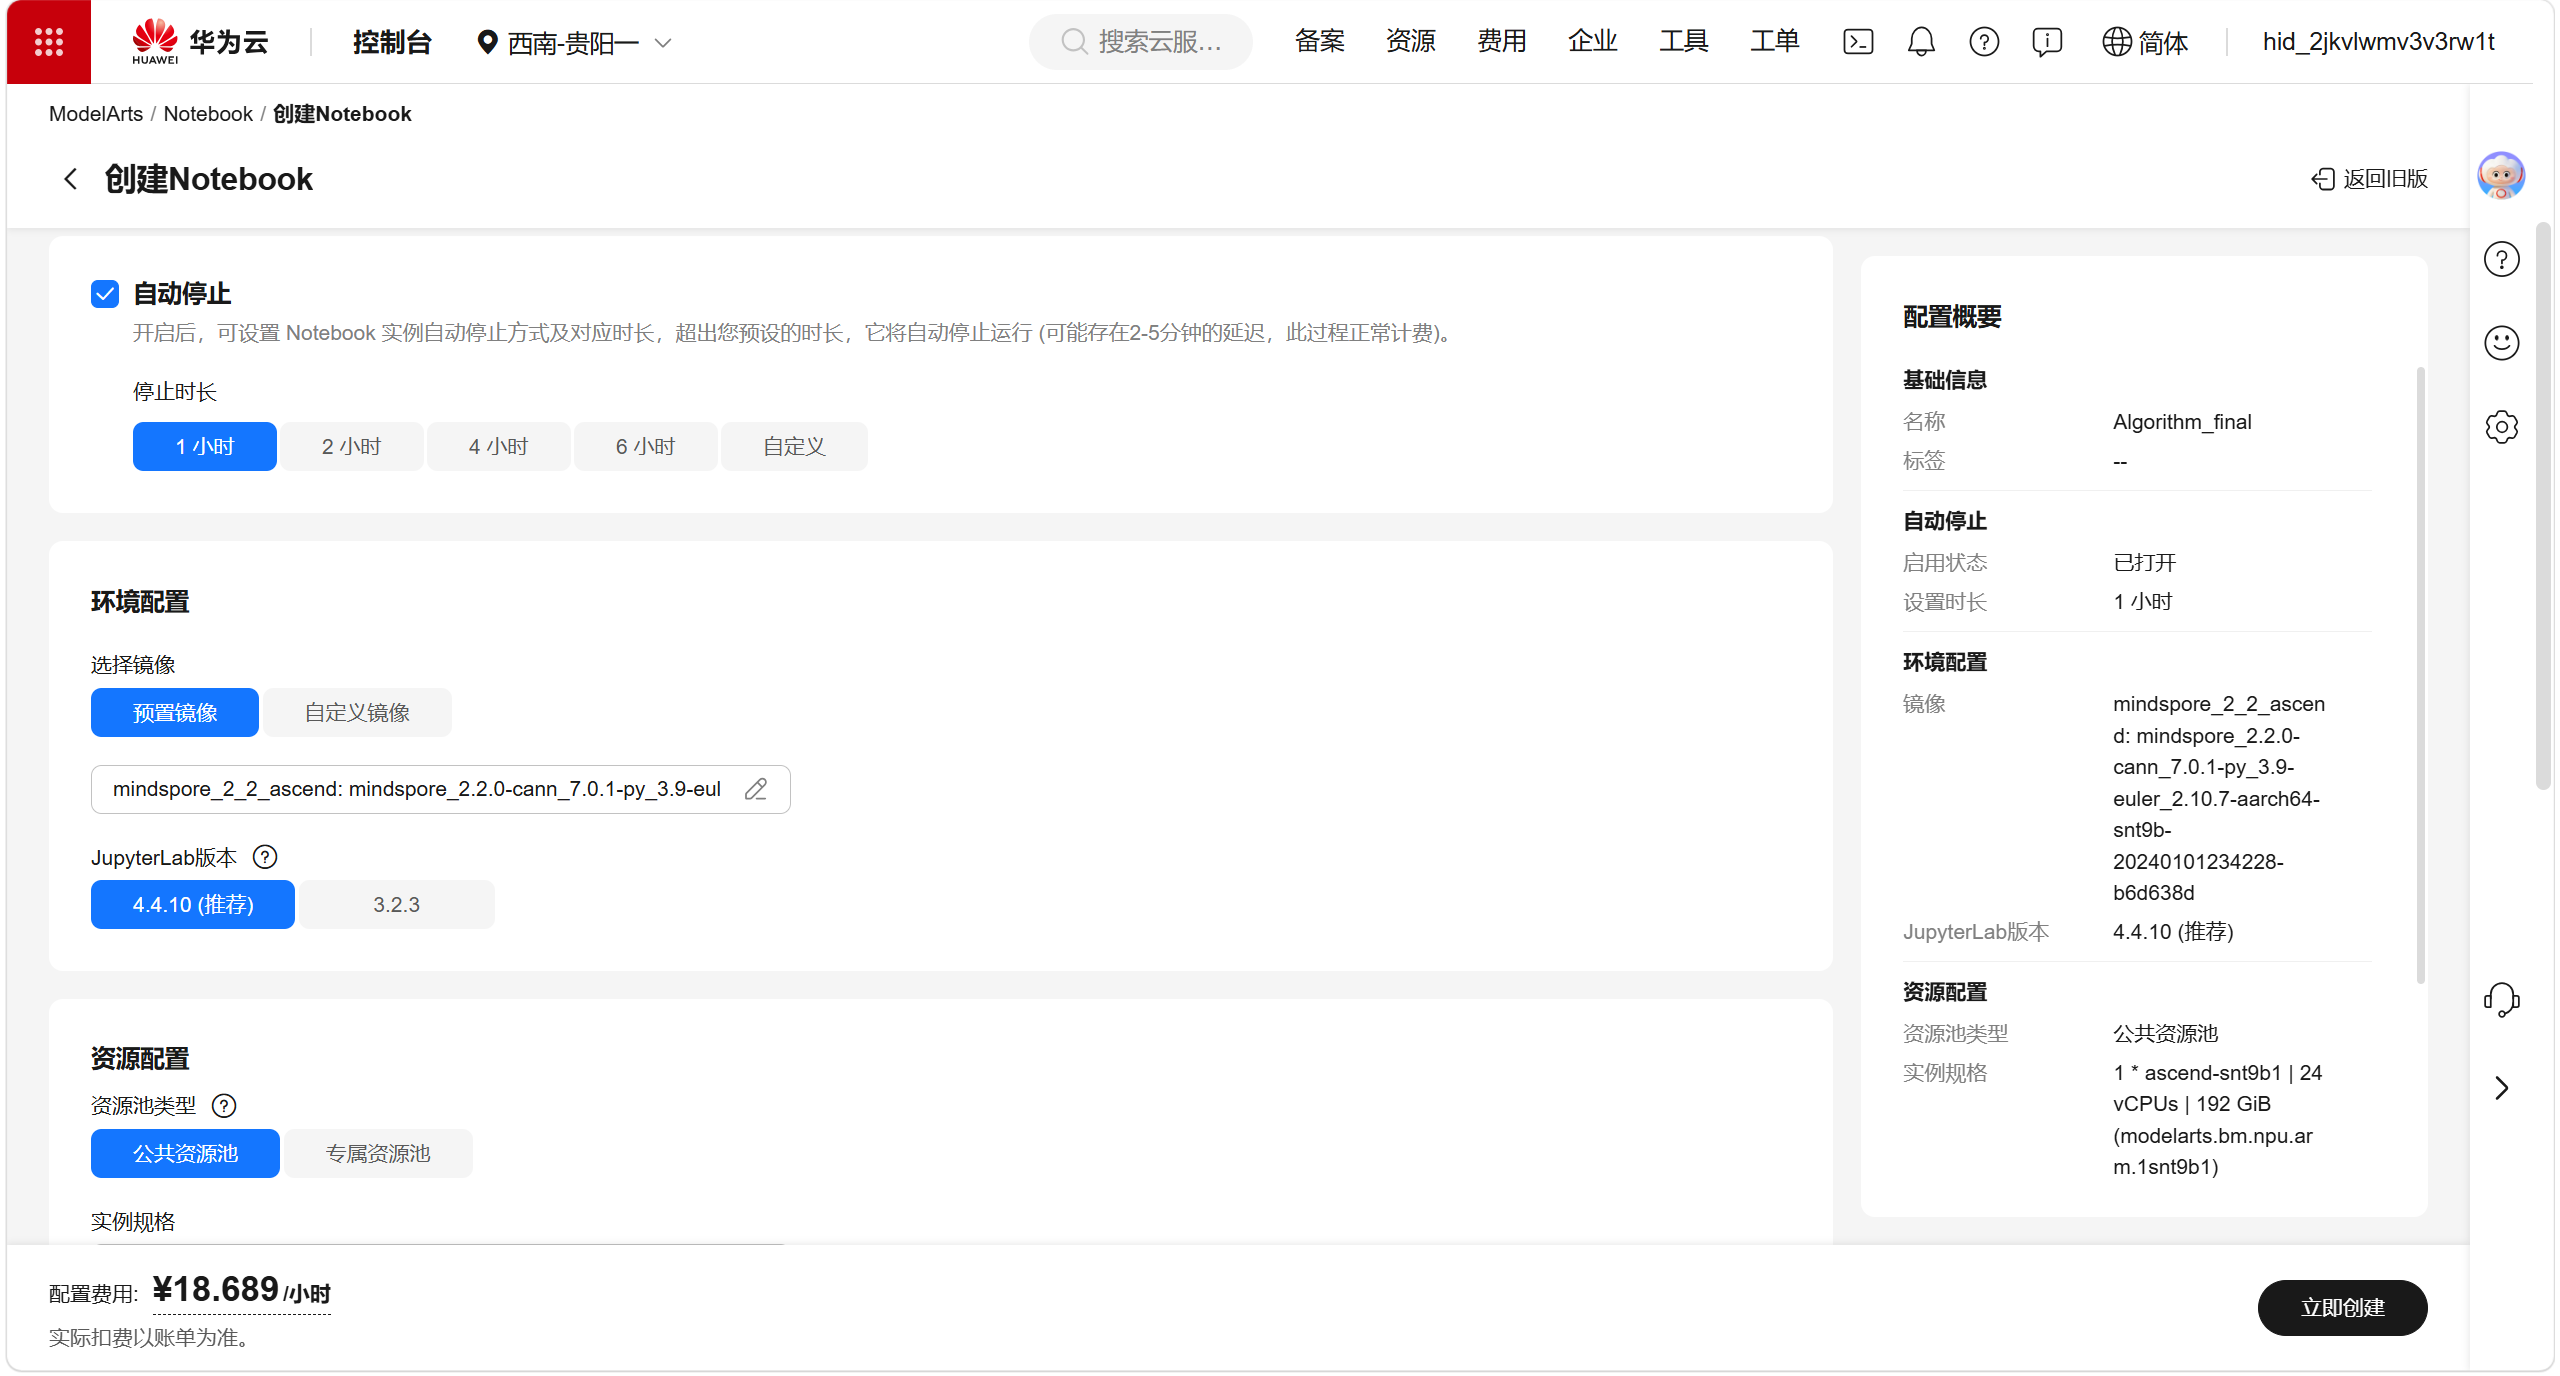
\includegraphics[width=0.84\textwidth]{01_ModelArts环境_创建Notebook配置.png}
  \caption{华为云 ModelArts Notebook 创建与环境配置}
  \label{fig:modelarts-config}
\end{figure}

\section{实验原理}

\subsection{MNIST 数据集}

MNIST 是经典的手写数字图像数据集，由 0 到 9 共 10 类灰度数字图像组成。根据实验指导书，训练集包含 60000 张图片，测试集包含 10000 张图片，每张原始图像大小为 $28 \times 28$。本次实验在预处理阶段将图像调整为 $32 \times 32$，使其更适合 LeNet-5 的卷积和池化结构。

\subsection{卷积神经网络}

卷积神经网络（Convolutional Neural Network, CNN）是一类常用于图像处理的深度学习模型。它通过卷积层提取局部特征，通过池化层降低特征图尺寸并增强一定的平移鲁棒性，最后再使用全连接层完成分类。在手写数字识别任务中，卷积层可以学习数字笔画边缘、局部形状和组合结构，全连接层则根据这些特征输出 10 个数字类别的预测结果。

\subsection{LeNet-5 网络结构}

LeNet-5 是较早用于手写数字识别的卷积神经网络结构。本次实验中的原始 LeNet-5 由两个卷积层、两个最大池化层和三个全连接层组成。输入图像通道数为 1，第一层卷积输出通道数为 6，第二层卷积输出通道数为 16；经过展平后，特征依次进入输出维度为 120、84 和 10 的全连接层。实验代码中使用 ReLU 激活函数和最大池化层，以提升非线性表达能力和训练效果。

\subsection{损失函数、优化器与评价指标}

实验中使用 \texttt{SoftmaxCrossEntropyWithLogits} 作为损失函数。该损失函数适用于多分类任务，可以将模型输出的 logits 与真实标签进行比较，并计算交叉熵损失。由于 MNIST 标签为单一类别编号，代码中设置 \texttt{sparse=True}，并使用 \texttt{reduction='mean'} 对批次损失取平均值。

优化器采用 \texttt{Momentum}，学习率设置为 0.01，动量系数设置为 0.9。Momentum 在梯度下降的基础上引入历史梯度方向，有助于加快收敛并减小训练过程中的震荡。评价指标采用 Accuracy，即测试集中预测正确样本数占总样本数的比例。平均损失值（Avg loss）用于反映模型在测试集上的整体误差水平。

\section{实验过程}

\subsection{创建并打开 ModelArts Notebook}

首先在华为云 ModelArts 控制台创建 Notebook，区域选择“西南-贵阳一”，镜像选择 MindSpore 2.2 的 Ascend+ARM 预置镜像，JupyterLab 版本使用 4.4.10。Notebook 创建完成并进入运行状态后，通过 JupyterLab 打开老师提供的源代码 notebook，即 \texttt{src/LeNet-mnist\_run.ipynb}，并在 \texttt{/home/ma-user/work} 工作目录中按顺序运行各个代码单元。ModelArts Notebook 创建配置见图~\ref{fig:modelarts-config}。

\subsection{运行数据准备代码}

源代码前半部分已经给出了实验所需的数据准备流程，因此实验时主要按照 notebook 顺序运行相应代码单元。首先安装 \texttt{download} 库并配置 no\_proxy 环境变量，随后从 MindSpore 官方提供的对象存储地址下载 \texttt{MNIST\_Data.zip}，并解压到当前工作目录。下载过程显示数据文件大小约为 10.3 MB，解压完成后得到训练集和测试集目录。数据集下载成功截图如图~\ref{fig:mnist-download} 所示。

\begin{figure}[H]
  \centering
  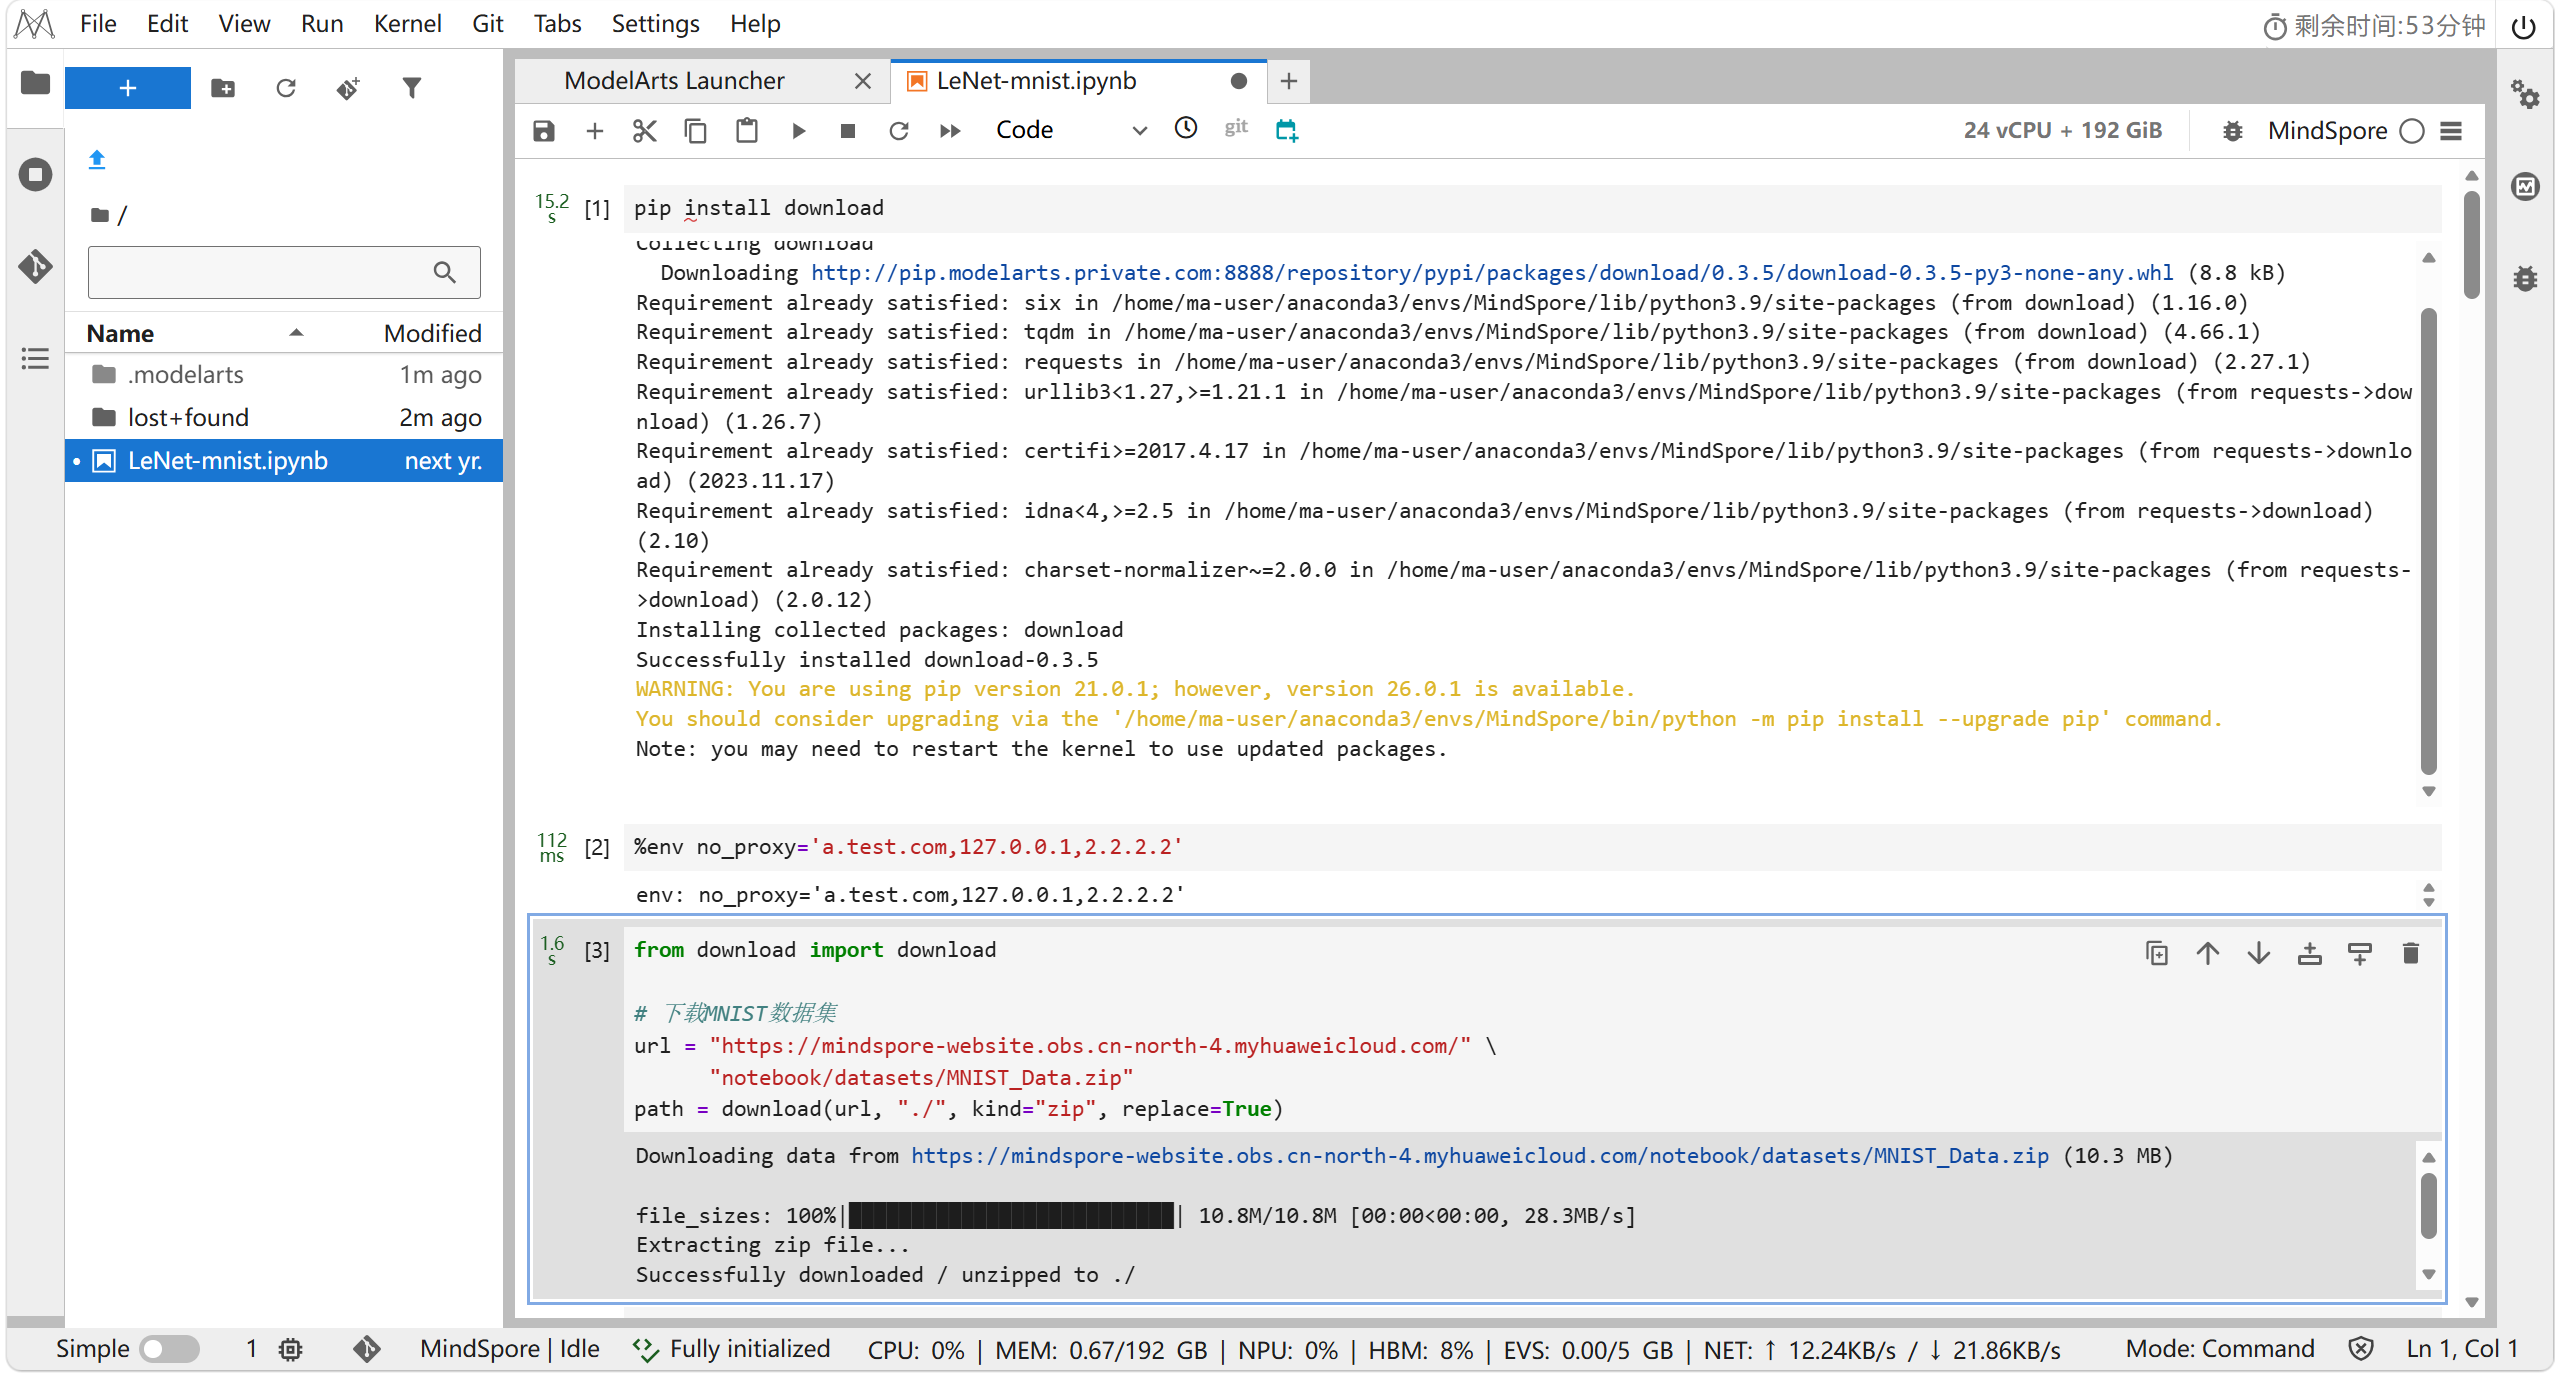
\includegraphics[width=0.86\textwidth]{02_MNIST数据集_下载解压成功.png}
  \caption{MNIST 数据集下载与解压成功}
  \label{fig:mnist-download}
\end{figure}

\subsection{运行环境设置与数据预处理}

完成数据下载后，继续运行 notebook 中的环境设置代码，导入 NumPy、Matplotlib、MindSpore 以及后续训练和可视化所需模块，并将运行设备设置为 Ascend。相关代码截图如图~\ref{fig:import-modules} 所示。

\begin{figure}[H]
  \centering
  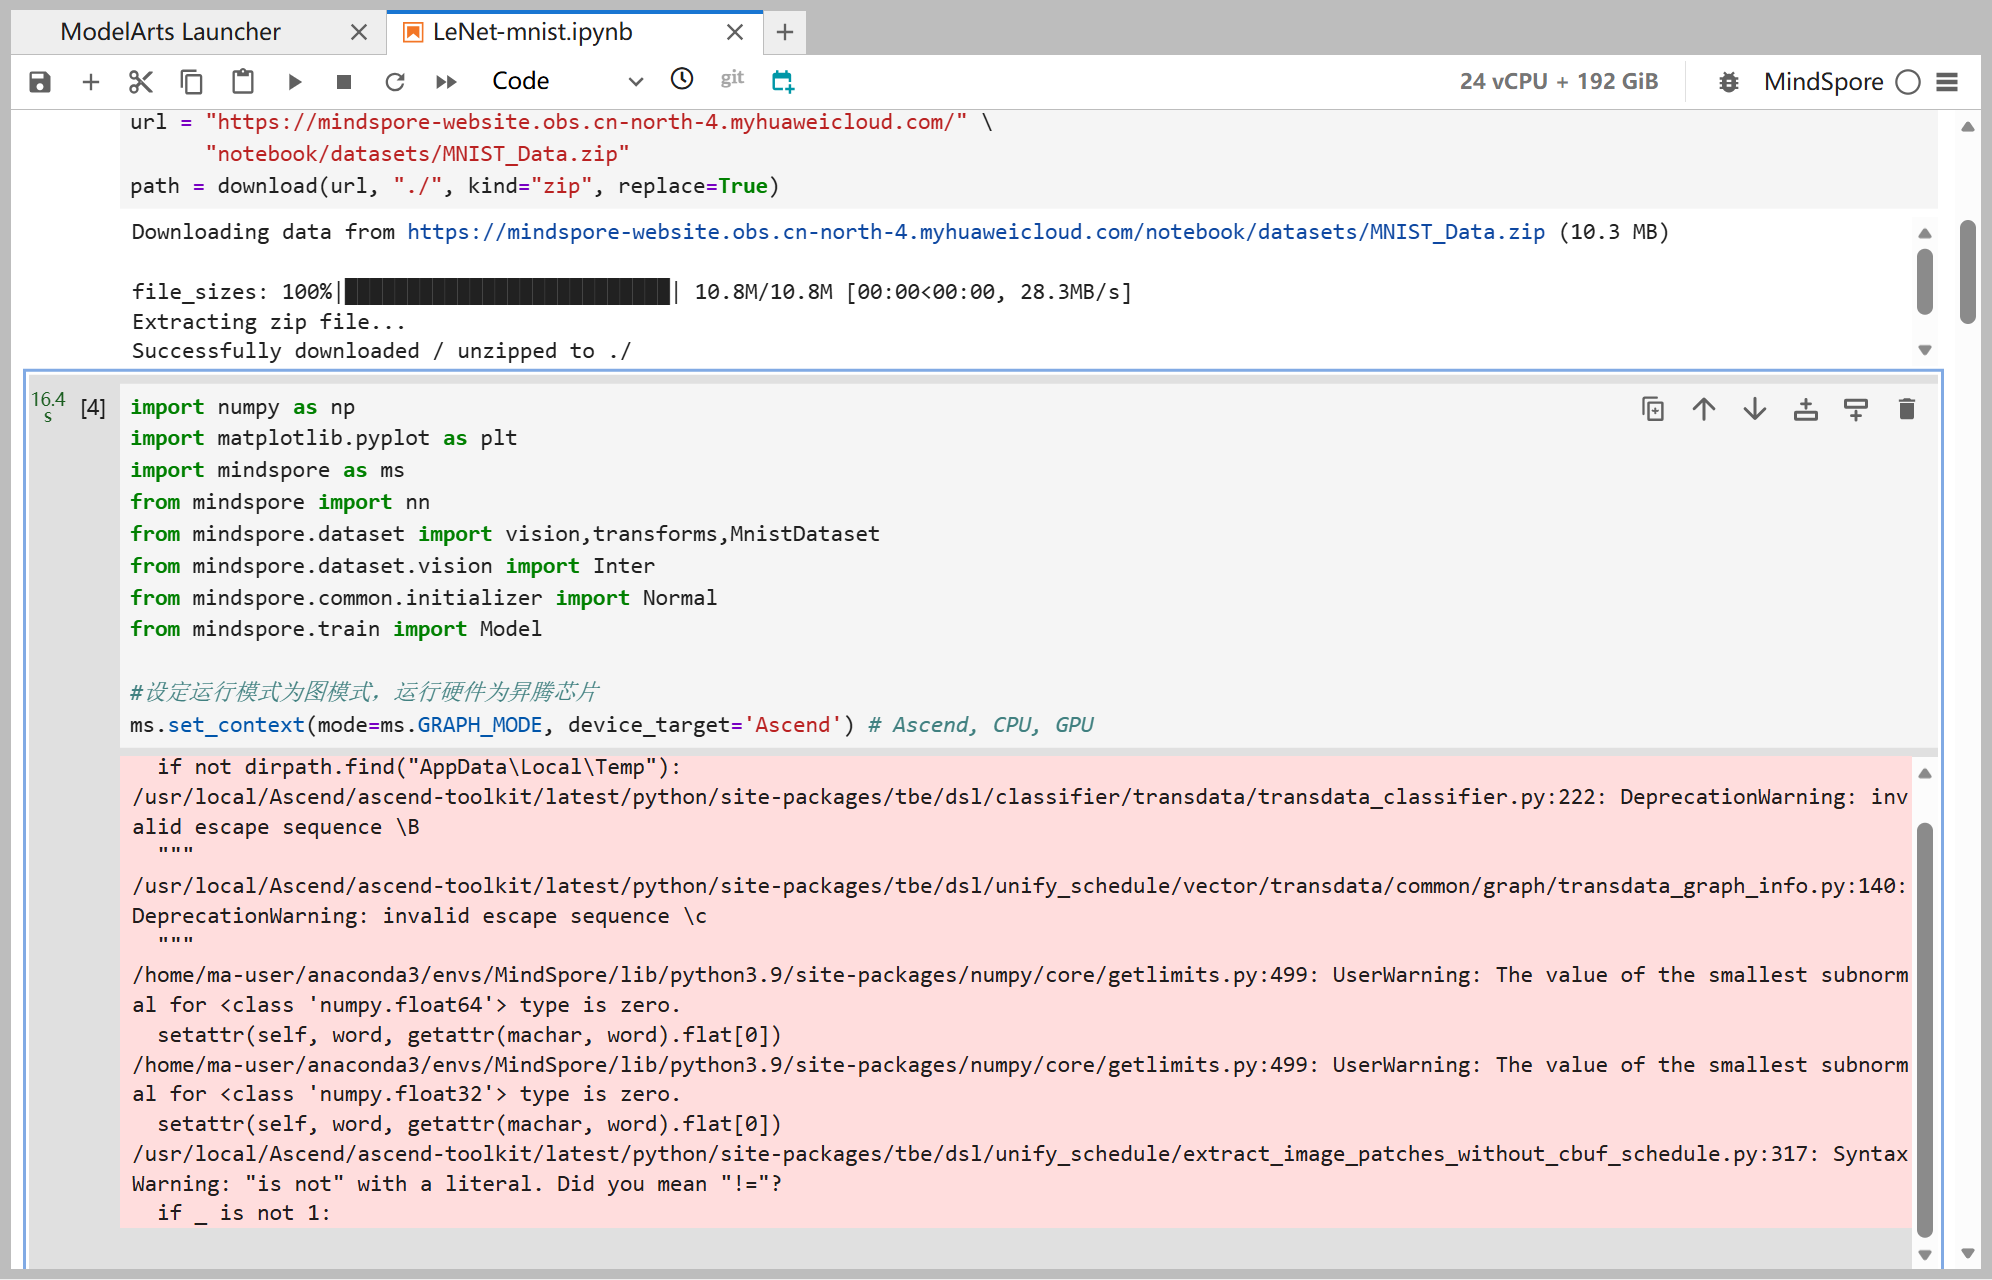
\includegraphics[width=0.86\textwidth]{03_导入Python库和MindSpore模块.png}
  \caption{导入 Python 库与 MindSpore 模块}
  \label{fig:import-modules}
\end{figure}

随后运行老师提供的数据读取与预处理代码。该部分代码将 MNIST 训练集和测试集读入后完成图像尺寸调整、像素值缩放、归一化、通道格式转换以及分批处理等操作，保证后续输入卷积神经网络的图像张量形状符合 LeNet-5 的训练要求。预处理代码如图~\ref{fig:datapipe} 所示。运行样本查看代码后，可以看到一个 batch 的图像张量形状为 $(32,1,32,32)$，并输出对应的样本图像与标签，结果如图~\ref{fig:sample-image} 所示。

\begin{figure}[H]
  \centering
  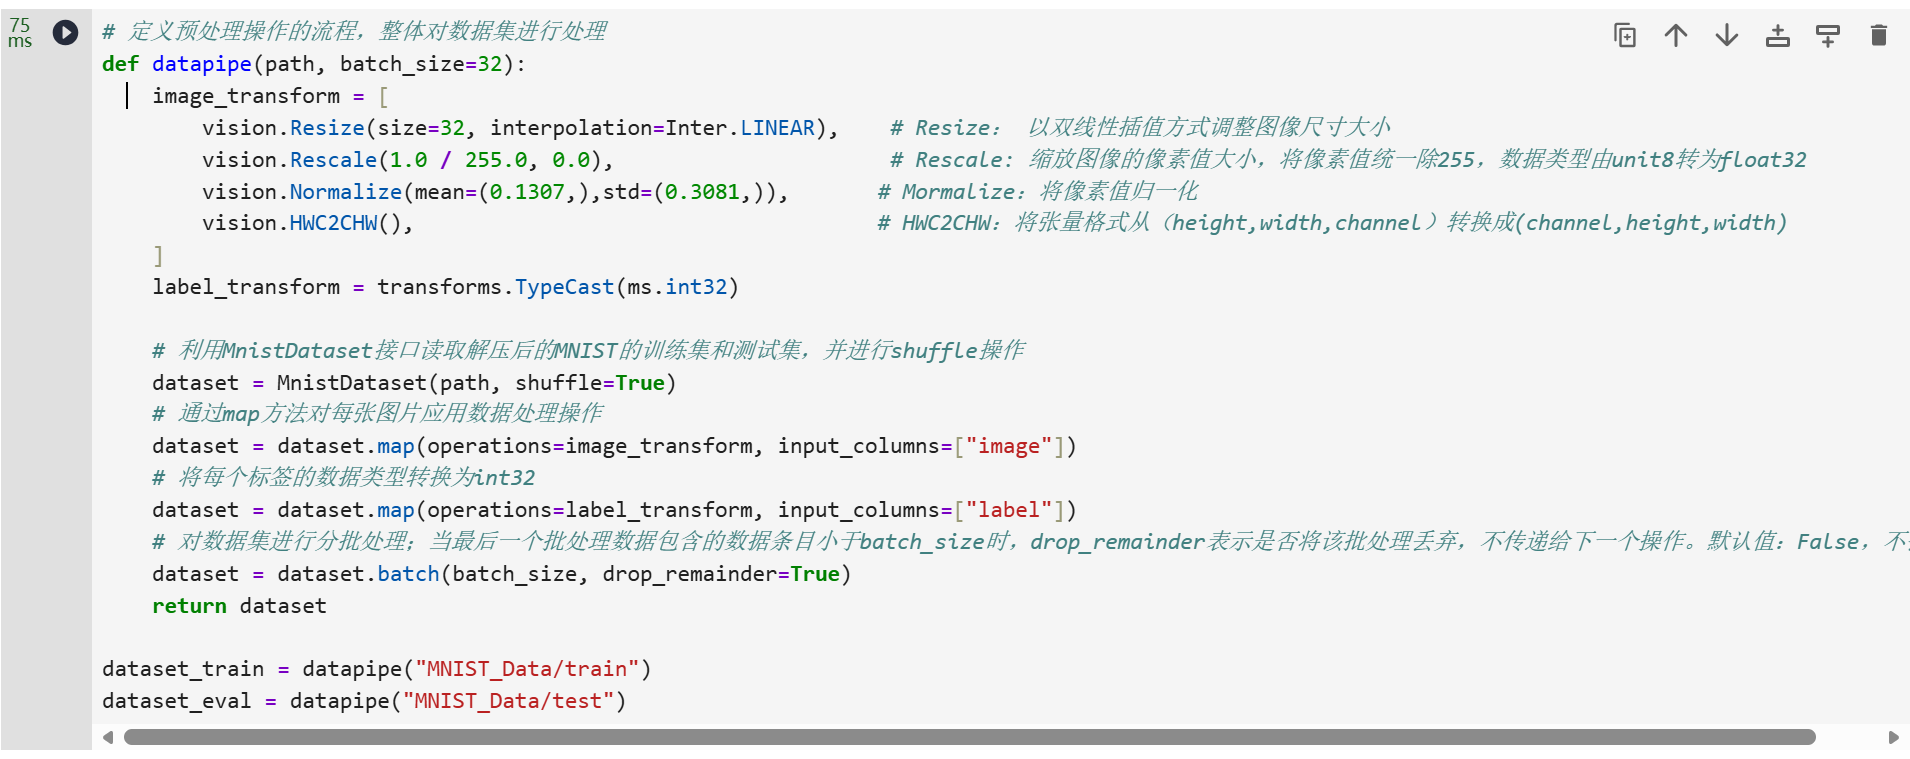
\includegraphics[width=0.95\textwidth]{04_读取数据集并完成预处理.png}
  \caption{MNIST 数据读取与预处理流程}
  \label{fig:datapipe}
\end{figure}

\begin{figure}[H]
  \centering
  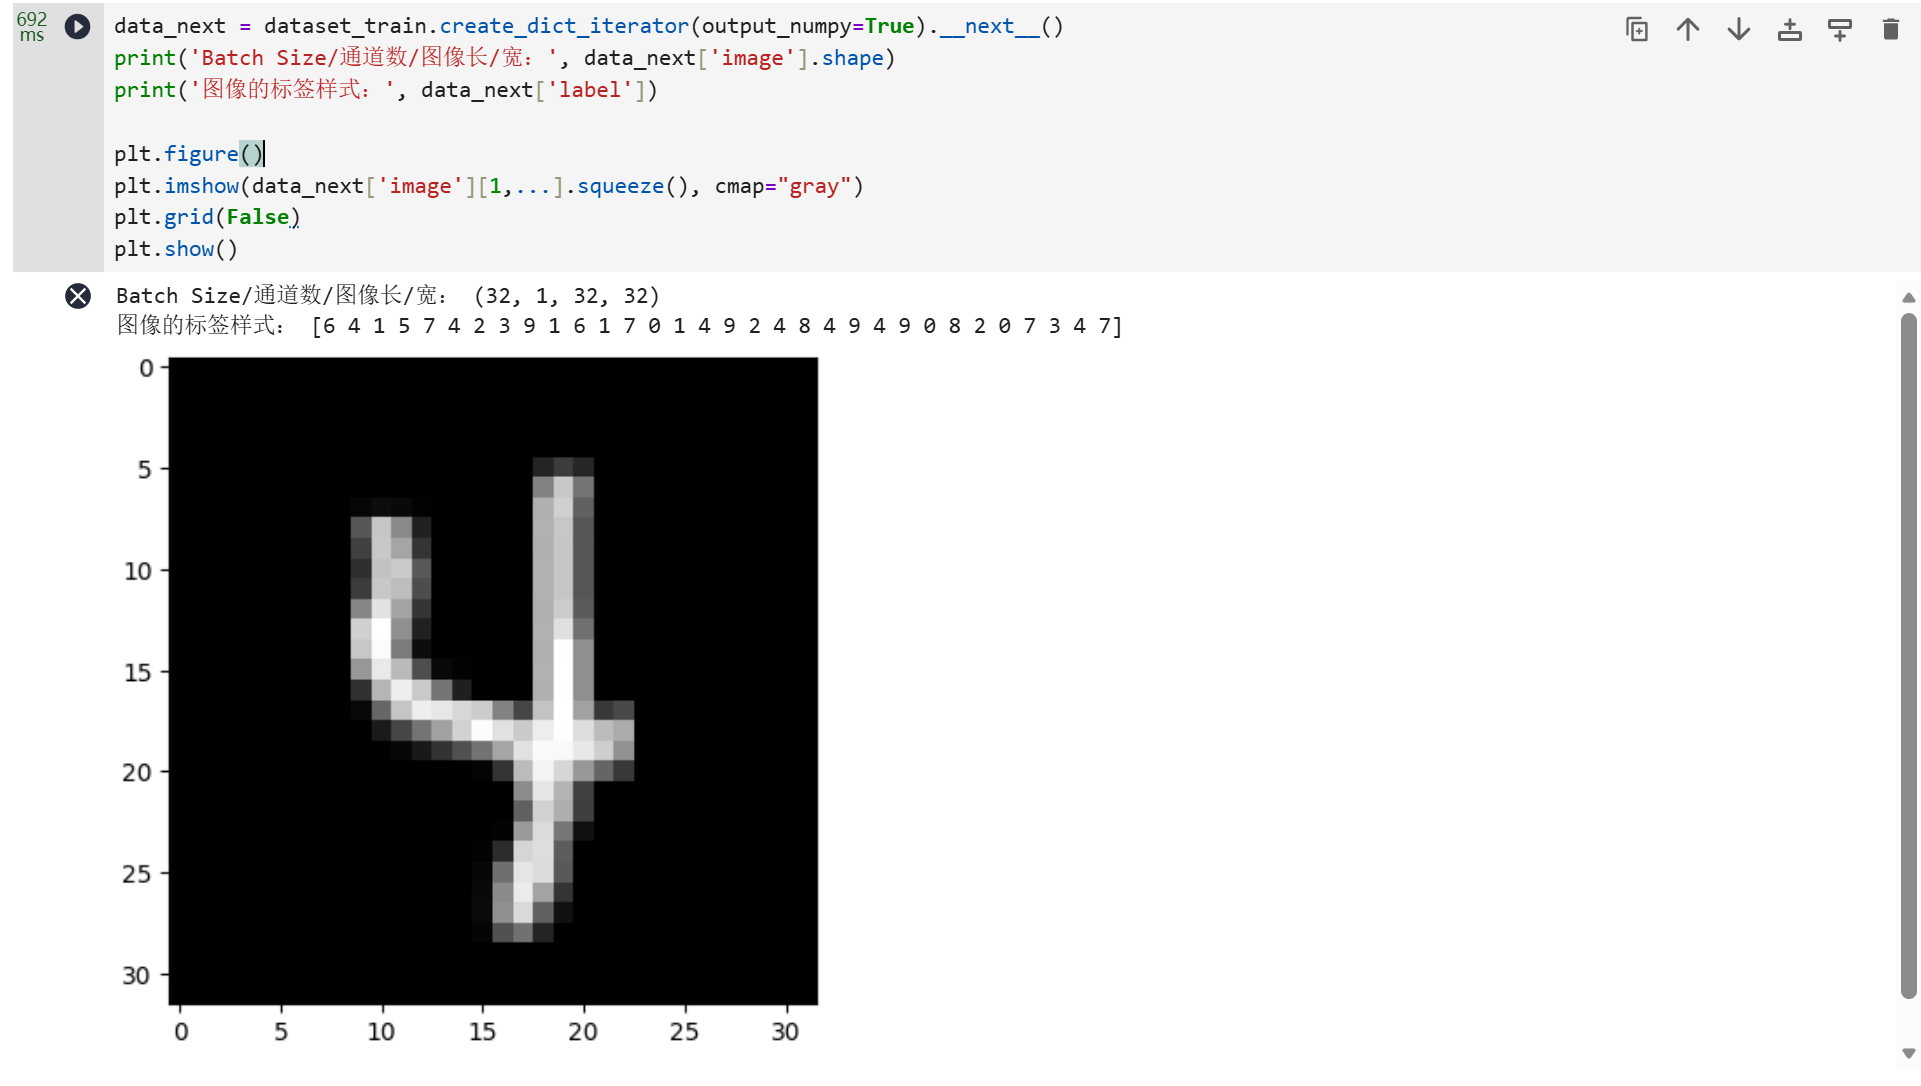
\includegraphics[width=0.82\textwidth]{04_读取任意一个数据内容.png}
  \caption{MNIST 样本图像与标签输出}
  \label{fig:sample-image}
\end{figure}

\subsection{构建原始 LeNet-5 并训练}

原始 LeNet-5 卷积神经网络结构已经在老师提供的 notebook 中给出。实验中直接运行对应代码单元，完成网络类定义、模型实例化、损失函数和优化器配置。原始网络结构代码如图~\ref{fig:lenet-code} 所示。

\begin{figure}[H]
  \centering
  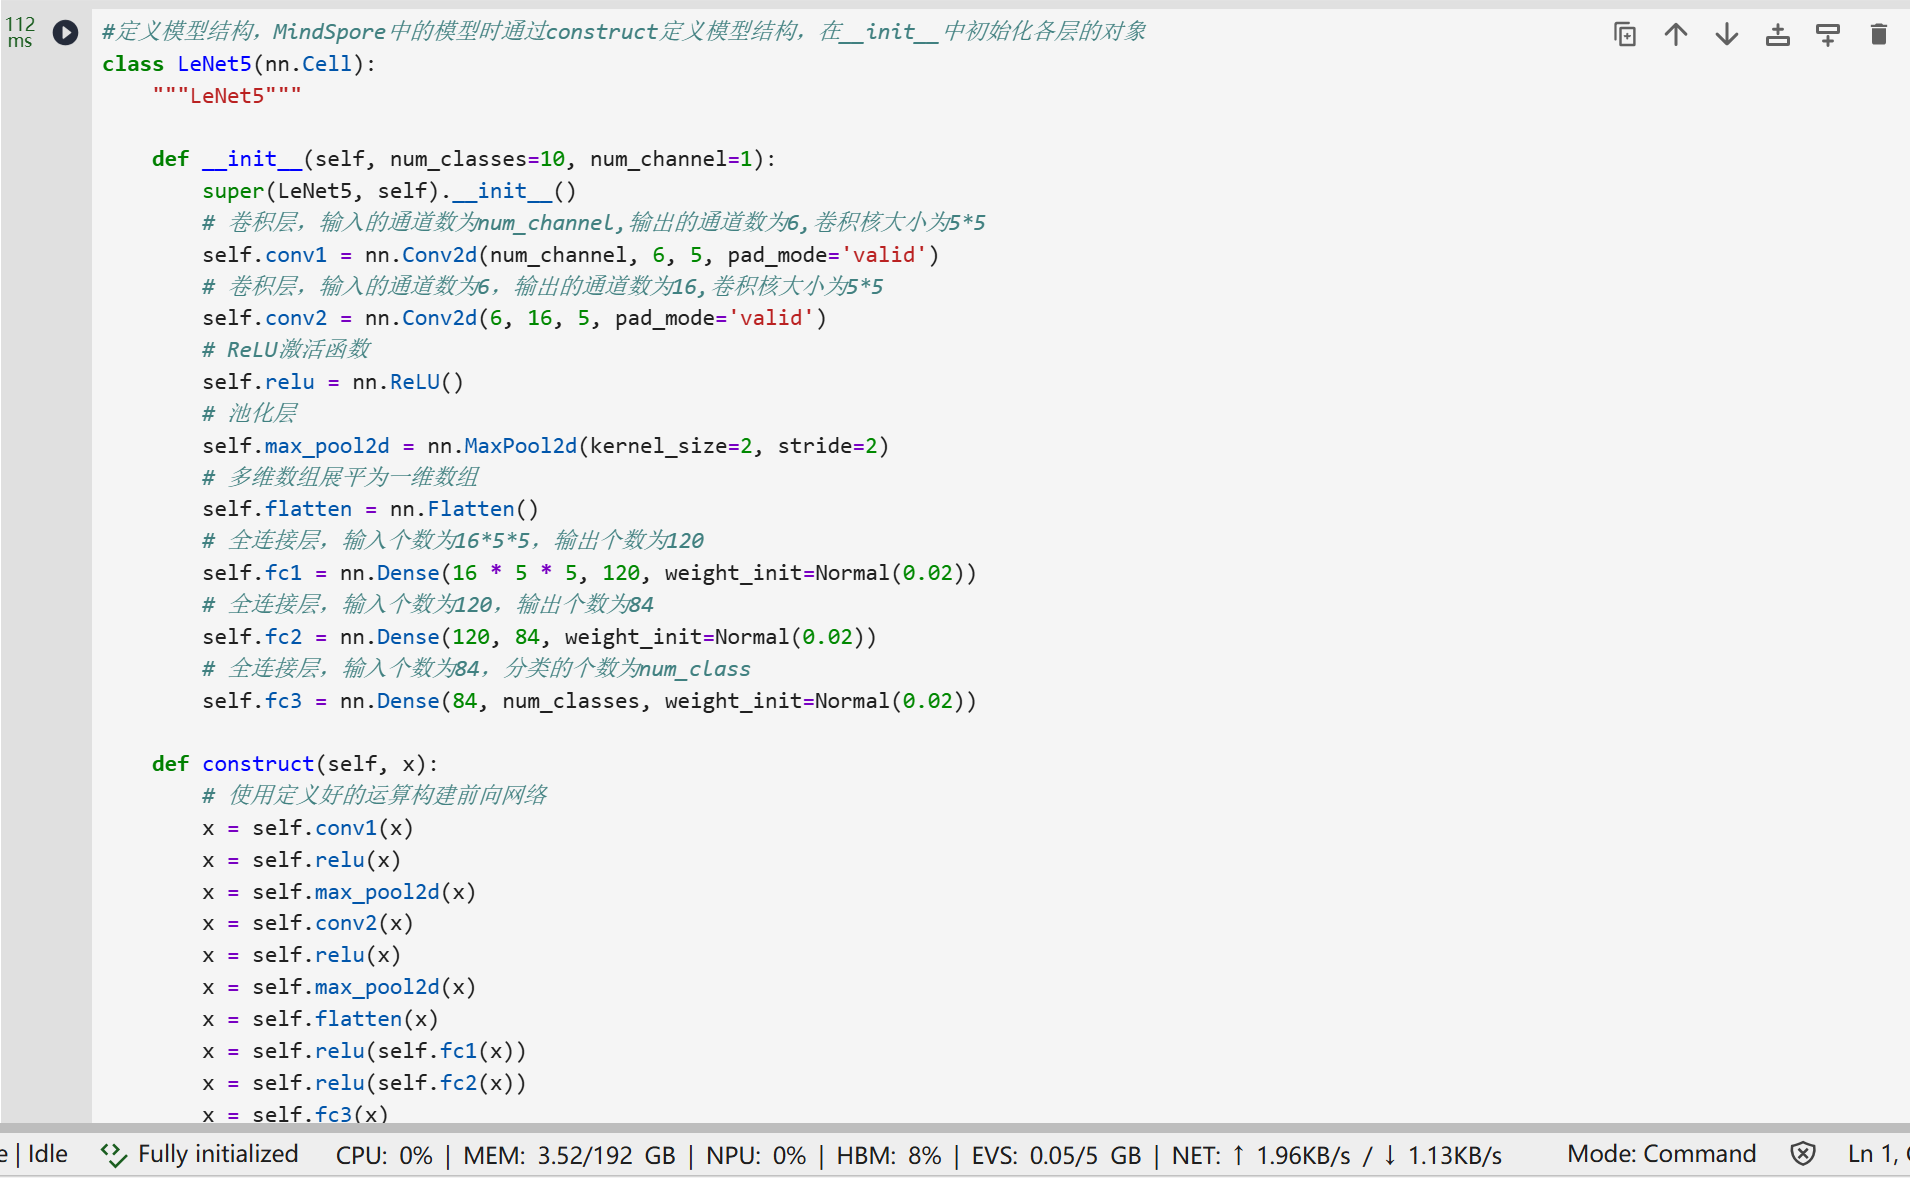
\includegraphics[width=0.84\textwidth]{05_构建LeNet5卷积神经网络.png}
  \caption{原始 LeNet-5 网络结构代码}
  \label{fig:lenet-code}
\end{figure}

随后继续运行训练代码，卷积神经网络模型在 MNIST 训练集上训练 3 个 epoch，并在每轮训练结束后输出测试集上的 Accuracy 和 Avg loss。训练网络搭建过程如图~\ref{fig:train-code} 所示。

\begin{figure}[H]
  \centering
  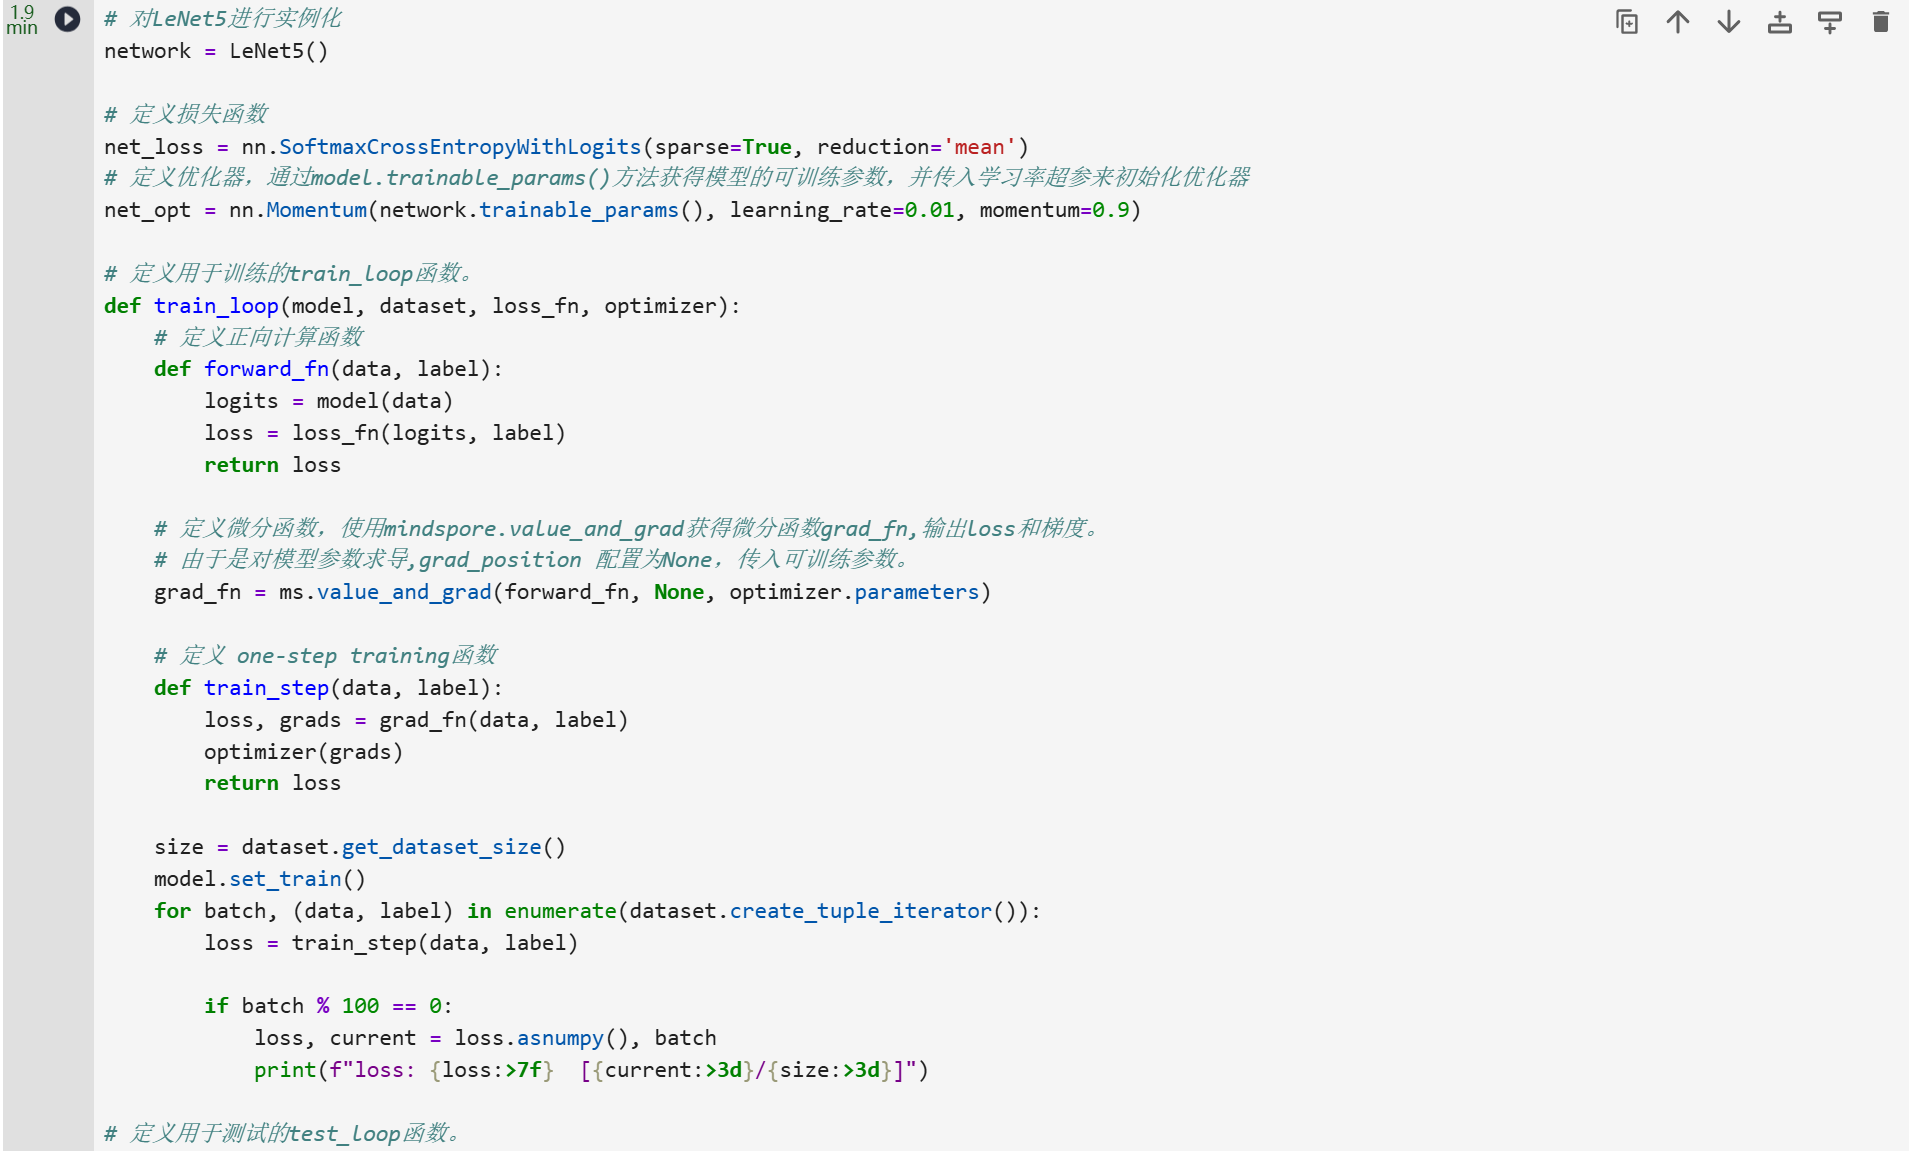
\includegraphics[width=0.84\textwidth]{06_搭建训练网络并进行训练.png}
  \caption{原始 LeNet-5 训练网络搭建与训练代码}
  \label{fig:train-code}
\end{figure}

\subsection{测试与预测可视化}

原始 LeNet-5 在第 1、2、3 轮训练后的测试准确率分别为 97.1\%、98.5\% 和 98.7\%。三轮训练输出如图~\ref{fig:original-epochs} 所示。可以看到，随着训练轮数增加，模型在测试集上的准确率逐步提升。

\begin{figure}[H]
  \centering
  \begin{minipage}[t]{0.31\textwidth}
    \centering
    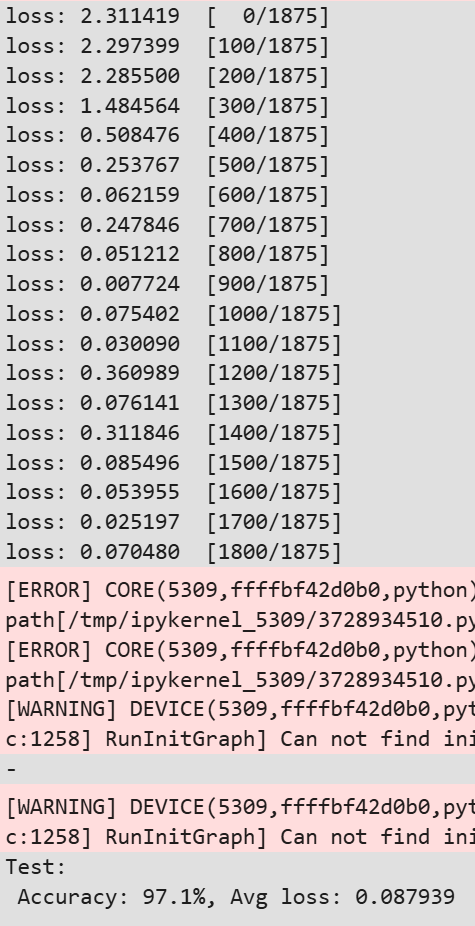
\includegraphics[width=\linewidth]{06_Epoch1训练结果_Accuracy97.1.png}
    \par\small (a) Epoch 1
  \end{minipage}
  \hfill
  \begin{minipage}[t]{0.31\textwidth}
    \centering
    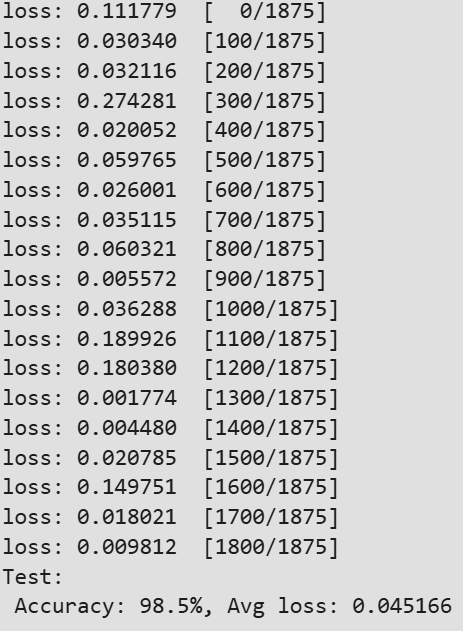
\includegraphics[width=\linewidth]{06_Epoch2训练结果_Accuracy98.5.png}
    \par\small (b) Epoch 2
  \end{minipage}
  \hfill
  \begin{minipage}[t]{0.31\textwidth}
    \centering
    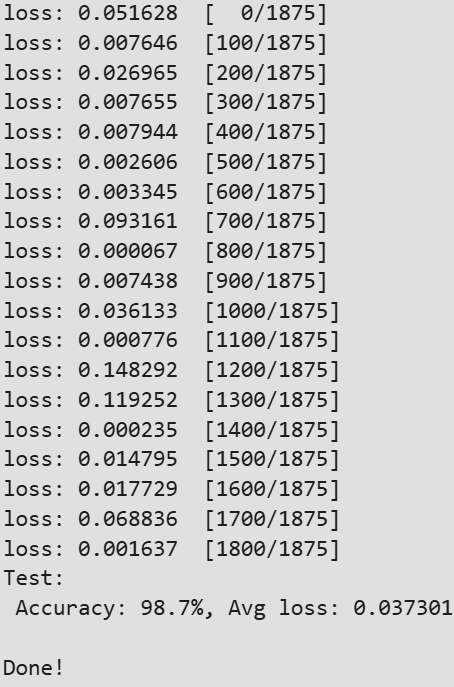
\includegraphics[width=\linewidth]{06_Epoch3最终训练结果_Accuracy98.7.png}
    \par\small (c) Epoch 3
  \end{minipage}
  \caption{原始 LeNet-5 三轮训练后的测试结果}
  \label{fig:original-epochs}
\end{figure}

完成训练后，继续运行 notebook 中的预测可视化代码。该部分从测试集中选取若干样本，加载训练后的模型参数并输出预测类别。预测可视化结果如图~\ref{fig:prediction-result} 所示，图像上方标题为模型预测结果。

\begin{figure}[H]
  \centering
  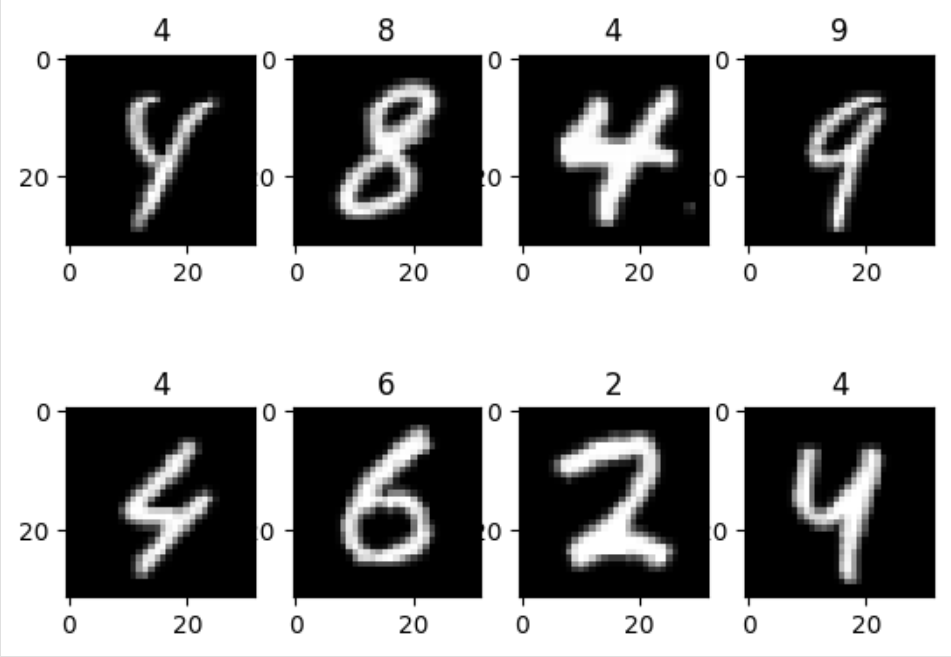
\includegraphics[width=0.62\textwidth]{07_result.png}
  \caption{原始 LeNet-5 对测试样本的预测可视化结果}
  \label{fig:prediction-result}
\end{figure}

\subsection{构建改进版 LeNet-5 并对比}

在完成老师提供的原始卷积神经网络实验后，进一步进行了改进版 LeNet-5 的对比实验。该部分不是重新设计完整训练流程，而是在原始 notebook 流程的基础上保持数据集、预处理方法、训练轮数、损失函数和优化器设置不变，仅调整 CNN 网络结构。改进版 LeNet-5 将两个卷积层输出通道数由原来的 6 和 16 调整为 8 和 32，同时将全连接层由 $120 \rightarrow 84$ 调整为 $128 \rightarrow 64$。最终采用的改进代码以 \texttt{src/改进版LeNet5代码.txt} 为准，完整代码统一放在附录中。

改进模型同样训练 3 个 epoch，每轮训练后记录测试准确率和平均损失值。改进模型第 1、2、3 轮训练后的测试准确率分别为 98.1\%、98.6\% 和 99.0\%，三轮训练输出如图~\ref{fig:improved-epochs} 所示。之后再将两组结果整理到表格和折线图中进行对比分析。

\begin{figure}[H]
  \centering
  \begin{minipage}[t]{0.31\textwidth}
    \centering
    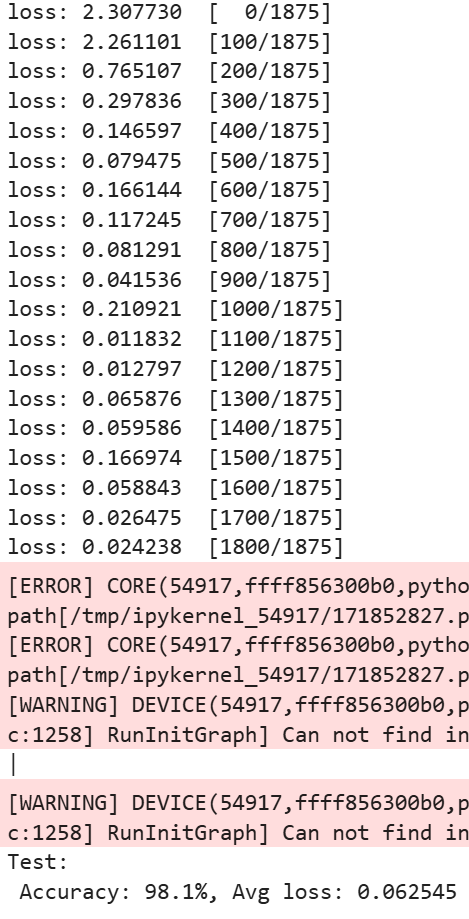
\includegraphics[width=\linewidth]{09_改进模型Epoch1训练结果_Accuracy98.1.png}
    \par\small (a) Epoch 1
  \end{minipage}
  \hfill
  \begin{minipage}[t]{0.31\textwidth}
    \centering
    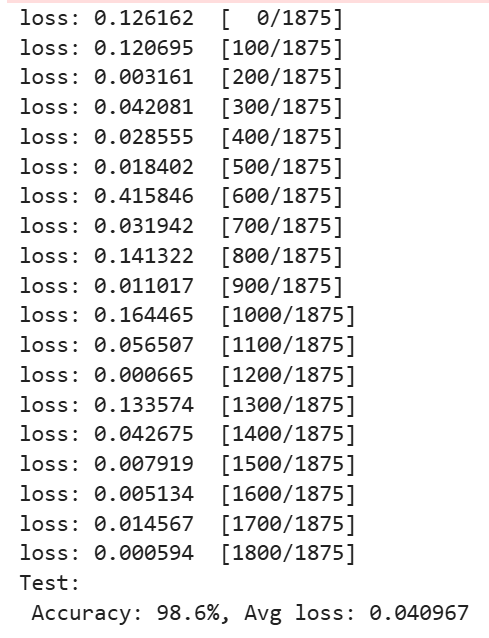
\includegraphics[width=\linewidth]{09_改进模型Epoch2训练结果_Accuracy98.6.png}
    \par\small (b) Epoch 2
  \end{minipage}
  \hfill
  \begin{minipage}[t]{0.31\textwidth}
    \centering
    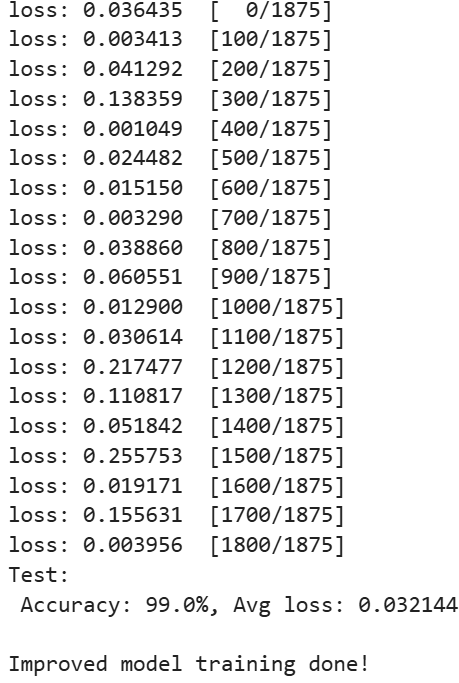
\includegraphics[width=\linewidth]{09_改进模型Epoch2训练结果_Accuracy99.0.png}
    \par\small (c) Epoch 3
  \end{minipage}
  \caption{改进版 LeNet-5 三轮训练后的测试结果}
  \label{fig:improved-epochs}
\end{figure}
\newpage
\section{实验数据与结果}

根据 notebook 输出和训练结果截图，原始 LeNet-5 的 3 轮训练测试结果整理如表~\ref{tab:original-result} 所示。

\begin{table}[htbp]
  \centering
  \caption{原始 LeNet-5 训练测试结果}
  \label{tab:original-result}
  \begin{tabular}{|c|c|c|}
    \hline
    训练轮次 & Accuracy & Avg loss \\
    \hline
    Epoch 1 & 97.1\% & 0.087939 \\
    Epoch 2 & 98.5\% & 0.045166 \\
    Epoch 3 & 98.7\% & 0.037301 \\
    \hline
  \end{tabular}
\end{table}

改进版 LeNet-5 的 3 轮训练测试结果如表~\ref{tab:improved-result} 所示。

\begin{table}[htbp]
  \centering
  \caption{改进版 LeNet-5 训练测试结果}
  \label{tab:improved-result}
  \begin{tabular}{|c|c|c|}
    \hline
    训练轮次 & Accuracy & Avg loss \\
    \hline
    Epoch 1 & 98.1\% & 0.062545 \\
    Epoch 2 & 98.6\% & 0.040967 \\
    Epoch 3 & 99.0\% & 0.032144 \\
    \hline
  \end{tabular}
\end{table}

两组实验的最终结果对比如表~\ref{tab:compare-result} 所示。

\begin{table}[htbp]
  \centering
  \caption{原始模型与改进模型最终结果对比}
  \label{tab:compare-result}
  \begin{tabular}{|c|c|c|c|c|}
    \hline
    模型 & 卷积通道数 & 全连接层结构 & 最终 Accuracy & 最终 Avg loss \\
    \hline
    原始 LeNet-5 & 6、16 & 120、84 & 98.7\% & 0.037301 \\
    改进版 LeNet-5 & 8、32 & 128、64 & 99.0\% & 0.032144 \\
    \hline
  \end{tabular}
\end{table}

从最终结果看，改进版 LeNet-5 相比原始模型准确率提升 0.3 个百分点，平均损失值降低 0.005157。在相同 epoch 数、相同损失函数和相同优化器条件下，改进结构的测试效果略好。

为了更直观地观察训练结果，改进版代码中加入了绘图程序，将原始模型和改进模型的三轮测试准确率、平均损失值以及最终结果对比保存为图片。准确率变化曲线如图~\ref{fig:accuracy-curve} 所示，平均损失变化曲线如图~\ref{fig:loss-curve} 所示，最终结果对比图如图~\ref{fig:final-comparison-chart} 所示。

\begin{figure}[H]
  \centering
  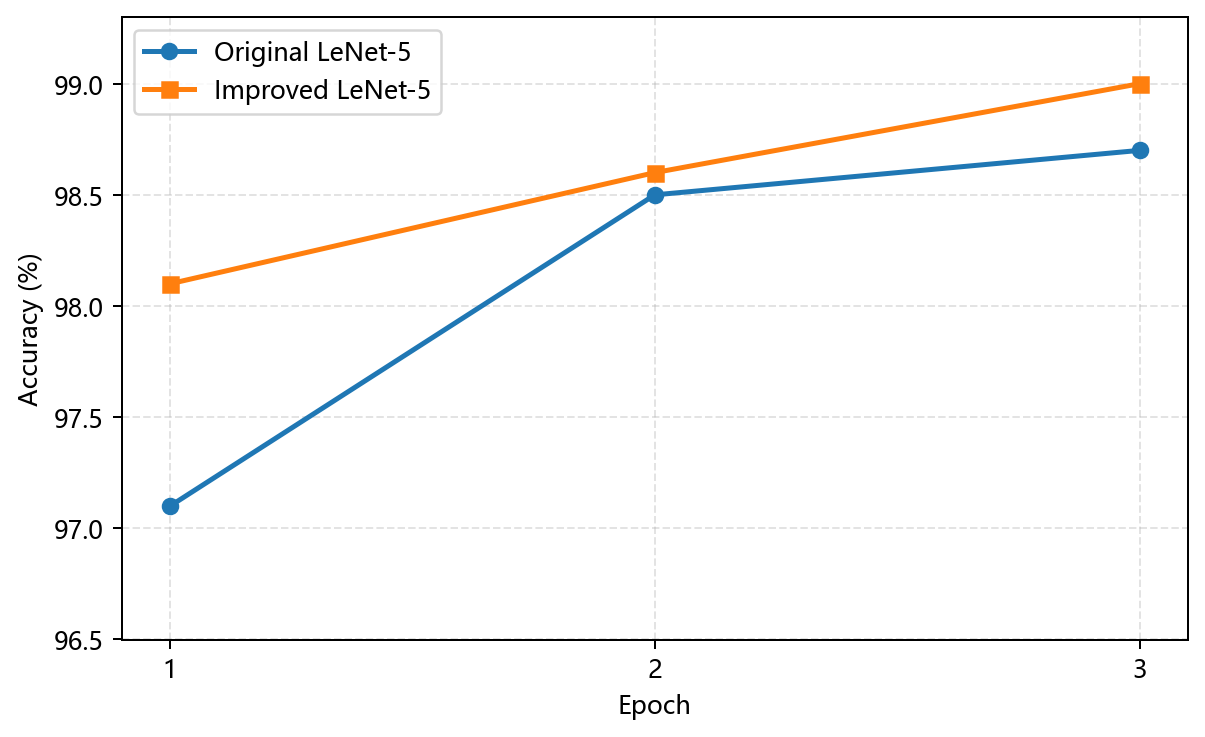
\includegraphics[width=0.70\textwidth]{10_accuracy_curve.png}
  \caption{原始模型与改进模型测试准确率变化曲线}
  \label{fig:accuracy-curve}
\end{figure}

\begin{figure}[H]
  \centering
  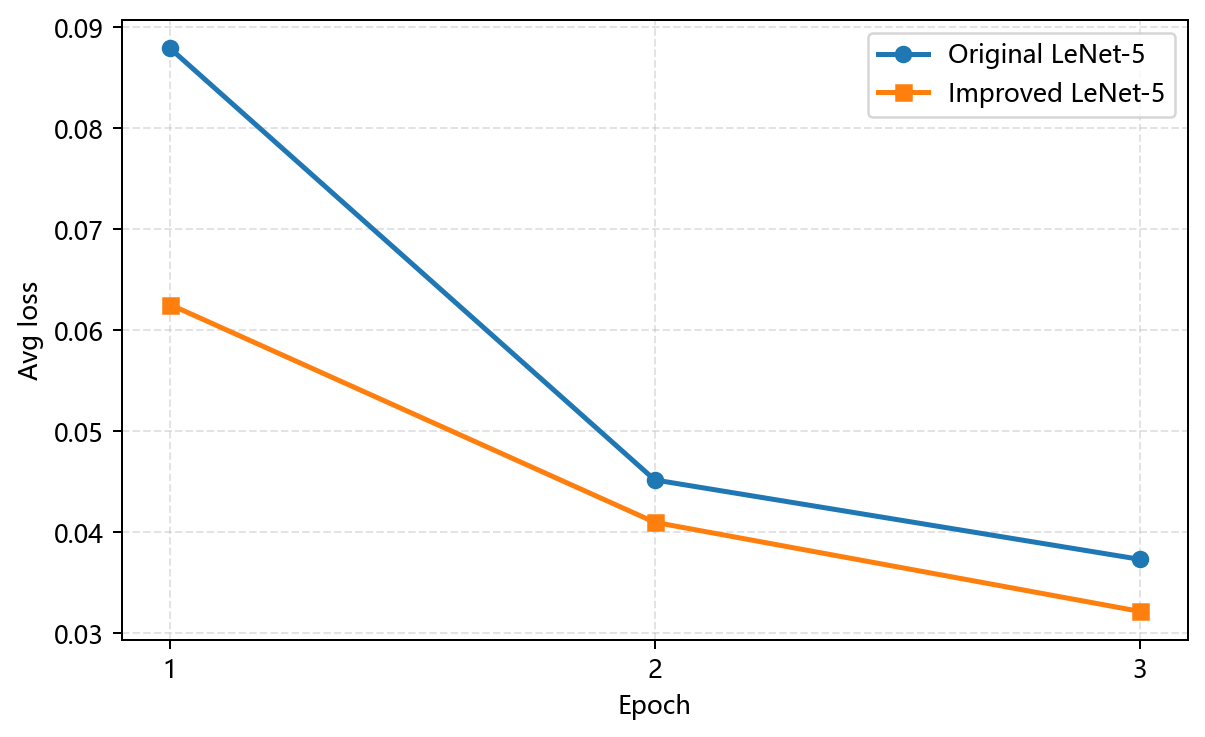
\includegraphics[width=0.70\textwidth]{11_loss_curve.png}
  \caption{原始模型与改进模型平均损失变化曲线}
  \label{fig:loss-curve}
\end{figure}

\begin{figure}[H]
  \centering
  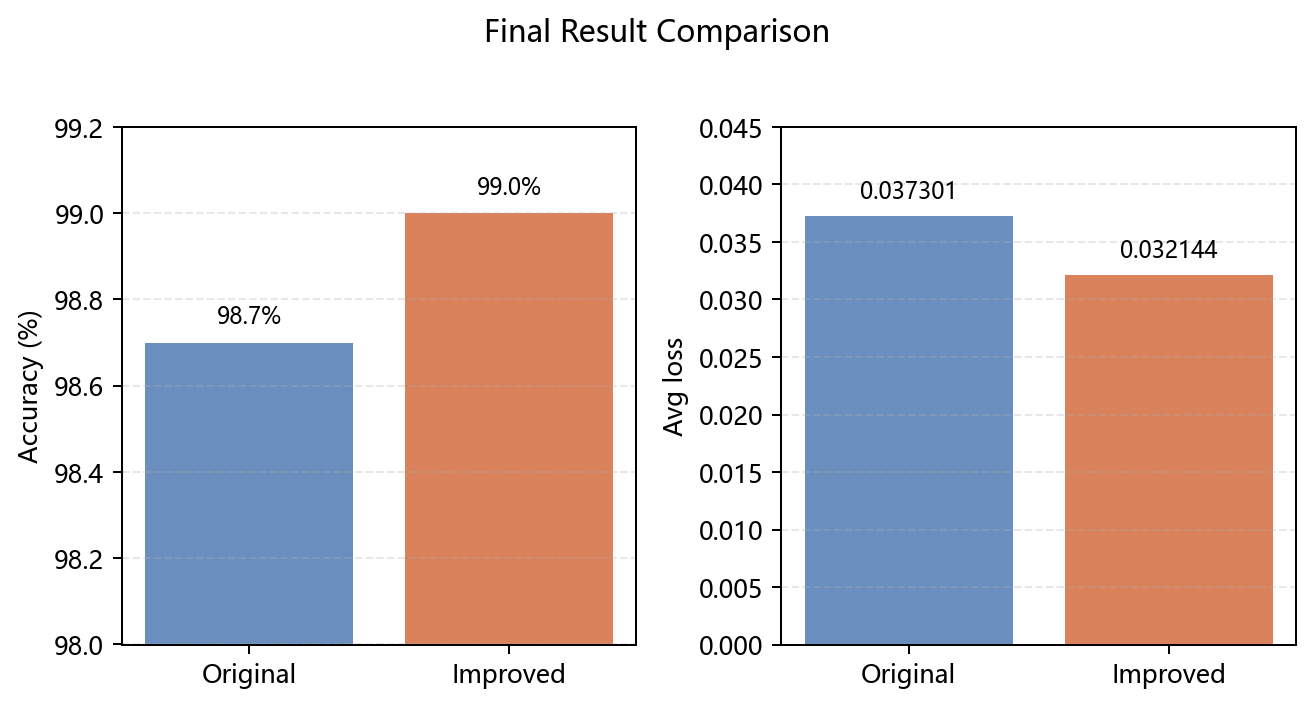
\includegraphics[width=0.76\textwidth]{12_final_comparison.png}
  \caption{原始模型与改进模型最终结果可视化对比}
  \label{fig:final-comparison-chart}
\end{figure}

\section{数据分析}

结合表~\ref{tab:original-result} 和图~\ref{fig:accuracy-curve}，原始 LeNet-5 随着 epoch 增加，测试准确率从 97.1\% 提升到 98.7\%，Avg loss 从 0.087939 下降到 0.037301。这个结果说明模型在训练过程中逐步学习到了 MNIST 数字图像中的有效特征，分类能力不断增强。虽然训练过程中单个 batch 的 loss 会因样本分布和随机初始化存在波动，但整体测试损失呈下降趋势，和深度学习模型训练的一般规律一致。

再结合表~\ref{tab:improved-result}、图~\ref{fig:loss-curve} 和图~\ref{fig:final-comparison-chart}，改进版 LeNet-5 在第 1 轮训练后就达到 98.1\% 的测试准确率，高于原始模型第 1 轮的 97.1\%。第 3 轮训练后，改进模型最终准确率达到 99.0\%，Avg loss 降低到 0.032144，两个指标都优于原始模型的最终结果。

改进模型性能提升的主要原因在于网络容量和特征提取能力有所增强。原始 LeNet-5 的卷积通道数为 6 和 16，改进后调整为 8 和 32，使网络可以在卷积阶段学习到更多局部特征图；同时，全连接层从 120、84 调整为 128、64，使分类层能够处理更丰富的高维特征表示。由于 MNIST 数据集本身较为规整，原始 LeNet-5 已经能够取得较高准确率，因此改进带来的提升幅度并不大，但在相同数据集、相同训练轮数、相同损失函数和相同优化器条件下，改进结构仍然获得了更高准确率和更低平均损失。

另外，模型准确率会受到参数初始化、数据 shuffle 顺序和训练环境等因素影响，单次实验结果可能存在一定随机波动。因此，本次分析主要在同一实验流程下比较两种结构的结果，用来分析适当增加卷积通道数和调整全连接层结构对 MNIST 测试表现的影响。


\section{实验总结}

本次实验中，我在华为云 ModelArts 平台上搭建了基于 MindSpore 2.2 的深度学习实验环境，完成了 MNIST 数据集下载、数据预处理、LeNet-5 卷积神经网络构建、模型训练、测试评估和预测可视化。通过完整运行 notebook，我熟悉了 MindSpore 中 \texttt{MnistDataset}、数据变换算子、\texttt{nn.Cell} 网络定义、自动微分训练流程、损失函数和优化器配置等基本用法。

从实验结果看，原始 LeNet-5 在 3 个 epoch 后测试准确率达到 98.7\%，已经能够较好地学习 MNIST 手写数字图像特征。在进一步改变神经网络结构后，改进版 LeNet-5 在相同训练条件下最终准确率达到 99.0\%，Avg loss 降低到 0.032144。对比这两组结果，我认为适当增加卷积通道数并调整全连接层结构可以提升模型表达能力。

通过这次实验，我对卷积神经网络的基本结构、MindSpore 模型训练流程、模型评估方法和网络结构改进方法有了更直观的理解。实验也存在不足：目前只在 MNIST 数据集上进行了验证，数据集规模和任务难度都比较有限。后续如果继续改进，可以尝试在更复杂的数据集上测试模型泛化能力，或者引入 Dropout、Batch Normalization、更深层卷积结构等方法。实验结束后，我也按照老师在课上提醒的要求及时停止或删除 ModelArts 环境，避免继续计费。

\newpage
\appendix
\section{改进版 LeNet-5 代码}

以下代码来自 \texttt{src/改进版LeNet5代码.txt}，用于定义改进版 LeNet-5 网络结构，完成模型训练与测试，并将训练结果图保存到 \texttt{figures} 文件夹。

\lstinputlisting[language=Python,basicstyle=\small\ttfamily,breaklines=true,columns=fullflexible]{src/改进版LeNet5代码.txt}

\end{document}
